% Section: Using Abisko
% Latex file for the MPI Course at HPC2N Umea 
%    Elaborated by P. Ojeda
%

%########################  NEW SECTION  ########################
\section{Linux terminal}

%%%%%%%%%%%%%%%%% NEW  SLIDE
\begin{frame}
	\frametitle{Linux OS}
	
        \begin{center}
        \includegraphics[width=6.5cm]{images/linux_os.png}
        \end{center}
\end{frame}

%%%%%%%%%%%%%%%%% NEW  SLIDE
\begin{frame}
	\frametitle{Linux OS}
	\begin{itemize}
		\item	UNIX-like OS 
		\item	used in modern Android smartphones
		\item   the difference between UNIX OS is small	
	\end{itemize}
	
\end{frame}

%%%%%%%%%%%%%%%%%%%%%%%%%%%%%%%%%%%%%%%%%%%%%%%%%%%%%%%%%%%%%%%%%%%%%%%%%%%%%%%%%%%%%
\begin{frame}
	\frametitle{Linux timeline}
        \begin{center}
        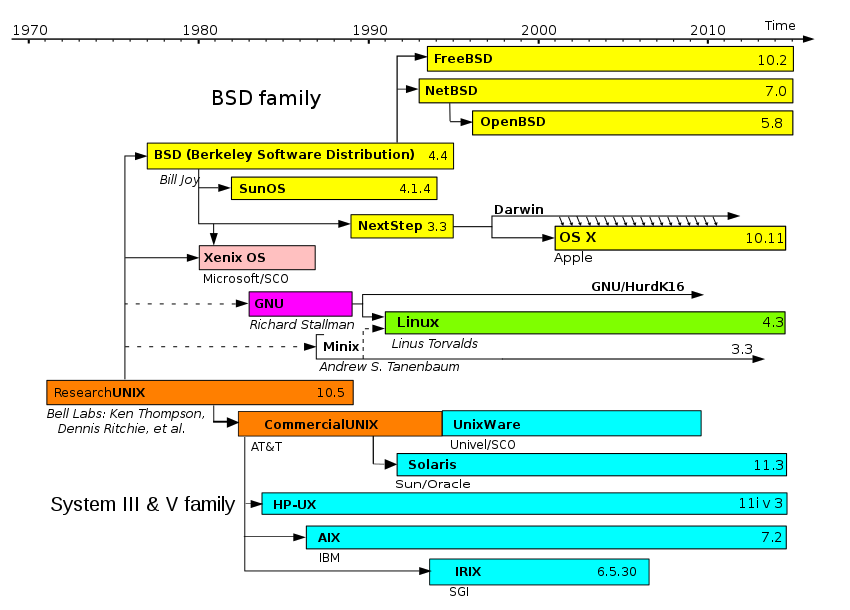
\includegraphics[width=8.6cm]{images/Unix_timeline.png}
        \end{center}
        {\tiny source: wikipedia}
\end{frame}

%%%%%%%%%%%%%%%%%%%%%%%%%%%%%%%%%%%%%%%%%%%%%%%%%%%%%%%%%%%%%%%%%%%%%%%%%%%%%%%%%%%%%
\begin{frame}
	\frametitle{The Linux terminal}
        \begin{center}
        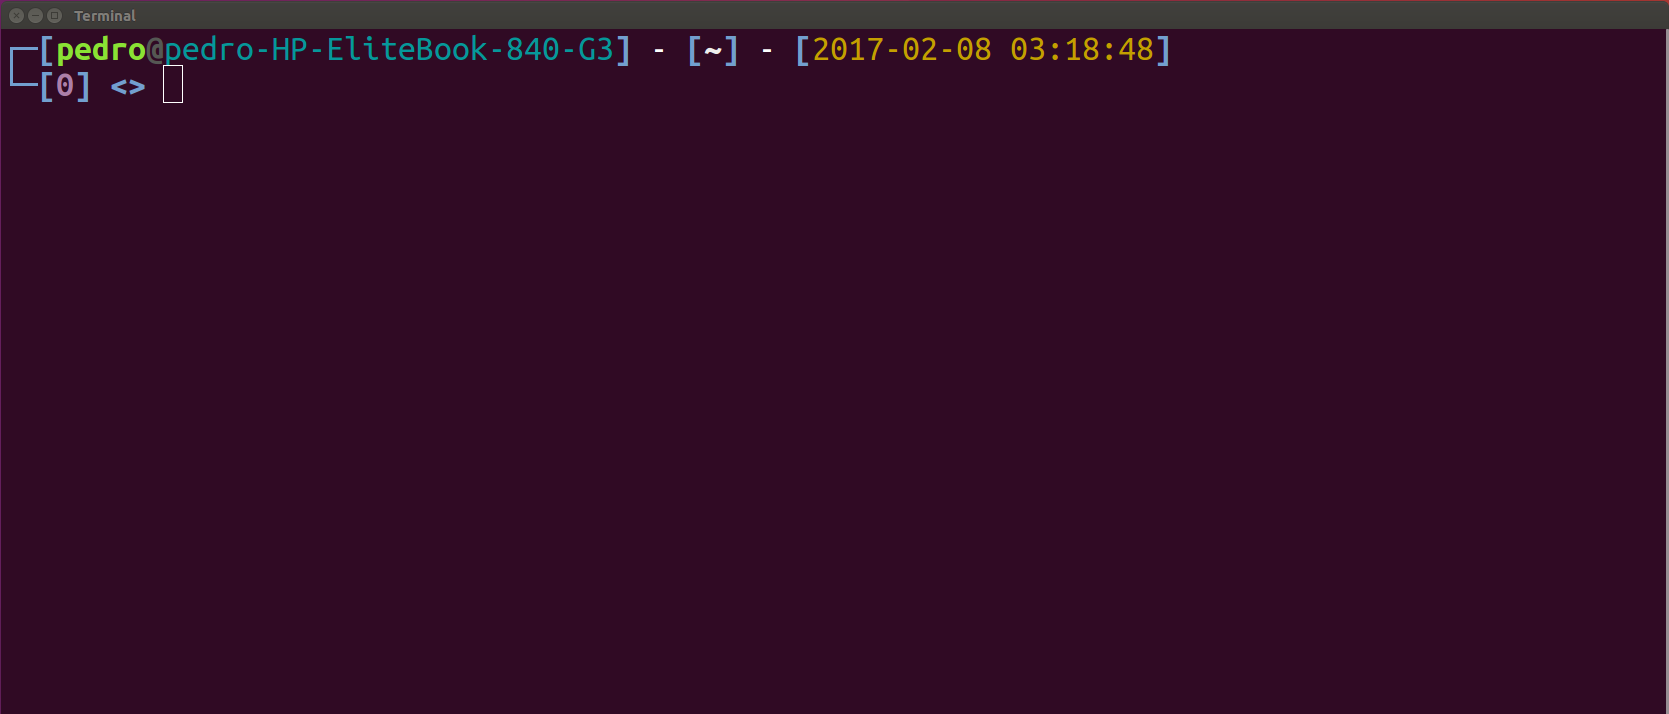
\includegraphics[width=9cm]{images/terminal_linux.png}
        \end{center}
	\begin{itemize}
		\item	on the terminal you can see the so-called Prompt
		\item	here you can control your PC/account or even
                 a remote server
	\end{itemize}
	
\end{frame}

%%%%%%%%%%%%%%%%%%%%%%%%%%%%%%%%%%%%%%%%%%%%%%%%%%%%%%%%%%%%%%%%%%%%%%%%%%%%%%%%%%%%%
\begin{frame}
	\frametitle{Files organization}
        \begin{center}
        \includegraphics[width=9.5cm]{images/tree_organization.png}
        \end{center}
\end{frame}

%%%%%%%%%%%%%%%%%%%%%%%%%%%%%%%%%%%%%%%%%%%%%%%%%%%%%%%%%%%%%%%%%%%%%%%%%%%%%%%%%%%%%
\begin{frame}[fragile]
	\frametitle{Useful commands: man}
        Manual pages. 
       
	\begin{itemize}
		\item \textbf{man command: man nano}
	\end{itemize}

{\tiny
	\begin{verbatim}
NANO(1)                     General Commands Manual                    NANO(1)

NAME
       nano - Nano's ANOther editor, an enhanced free Pico clone

SYNOPSIS
       nano [options] [[+line,column] file]...

DESCRIPTION
       nano  is  a small, free and friendly editor which aims to replace Pico,
       the default editor included in the non-free Pine package.   On  top  of
       copying  Pico's  look  and  feel, nano also implements some missing (or
       disabled by default) features in Pico, such as "search and replace" and
       "go to line and column number".
	\end{verbatim}
}
\end{frame}

%%%%%%%%%%%%%%%%%%%%%%%%%%%%%%%%%%%%%%%%%%%%%%%%%%%%%%%%%%%%%%%%%%%%%%%%%%%%%%%%%%%%%
\begin{frame}[fragile]
	\frametitle{Useful commands: ls}
List the content of a directory
{\scriptsize
	\begin{verbatim}
$ls
1CD9

$ls -l
total 24843644
drwxrwxr-x  2 pedro pedro        4096 nov  9 11:17 1CD9

$ls -la
total 24844368
drwxr-xr-x 44 pedro pedro        4096 feb 13 13:19 .
drwxr-xr-x  3 root  root         4096 sep 19 11:05 ..
drwxrwxr-x  2 pedro pedro        4096 nov  9 11:17 1CD9

$ls -lah
total 24G
drwxr-xr-x 44 pedro pedro 4,0K feb 13 13:25 .
drwxr-xr-x  3 root  root  4,0K sep 19 11:05 ..
drwxrwxr-x  2 pedro pedro 4,0K nov  9 11:17 1CD9
	\end{verbatim}
}

\end{frame}
%%%%%%%%%%%%%%%%%%%%%%%%%%%%%%%%%%%%%%%%%%%%%%%%%%%%%%%%%%%%%%%%%%%%%%%%%%%%%%%%%%%%%
\begin{frame}[fragile]
	\frametitle{Useful commands: ls}
{\scriptsize
	\begin{verbatim}
$ls -laht
total 24G
drwxr-xr-x 44 pedro pedro 4,0K feb 13 13:29 .
-rw-------  1 pedro pedro 431K feb 13 13:29 .zsh_history
drwx------  6 pedro pedro 4,0K feb 13 13:28 Linux_Abisko_Kebne

$ls -lahrt
total 24G
-rw-r--r--  1 pedro pedro  655 sep 19 11:05 .profile
	\end{verbatim}
}

\end{frame}

%%%%%%%%%%%%%%%%%%%%%%%%%%%%%%%%%%%%%%%%%%%%%%%%%%%%%%%%%%%%%%%%%%%%%%%%%%%%%%%%%%%%%
\begin{frame}[fragile]
	\frametitle{Useful commands: cd}
Change directory.

Useful cases:
	\begin{itemize}
        \item cd directory 

        move to "directory" 
        \item cd
 
         move to $\$HOME$ directory
        \item cd - 

        move to previous visited directory

        \item cd ..

        move to upper directory in the hierarchical tree
 
	\end{itemize}
        
\end{frame}

%%%%%%%%%%%%%%%%%%%%%%%%%%%%%%%%%%%%%%%%%%%%%%%%%%%%%%%%%%%%%%%%%%%%%%%%%%%%%%%%%%%%%
\begin{frame}
	\frametitle{Useful commands: cp}
        Copy files.

Useful cases:
	\begin{itemize}
        \item cp text.txt directory/

        copy text.txt file to "directory" 
        \item cp -r test/ directory/ 
 
        copy the directory test into directory/. 

        cp overwrites existing files!

	\end{itemize}
        

\end{frame}


%%%%%%%%%%%%%%%%%%%%%%%%%%%%%%%%%%%%%%%%%%%%%%%%%%%%%%%%%%%%%%%%%%%%%%%%%%%%%%%%%%%%%
\begin{frame}
	\frametitle{Useful commands: touch/mkdir}
        Create files.

Useful cases:
	\begin{itemize}
        \item touch text.txt

        creates text.txt file  
        \item mkdir test  
 
        creates the directory test 

	\end{itemize}

\end{frame}

%%%%%%%%%%%%%%%%%%%%%%%%%%%%%%%%%%%%%%%%%%%%%%%%%%%%%%%%%%%%%%%%%%%%%%%%%%%%%%%%%%%%%
\begin{frame}
	\frametitle{Useful commands: rm}
        Remove files.

Useful cases:
	\begin{itemize}
        \item rm text.txt

        deletes text.txt file  
        \item rm -rf test/  
 
        deletes the directory test 

        deleted files cannot be recovered!

	\end{itemize}
        

\end{frame}

%%%%%%%%%%%%%%%%%%%%%%%%%%%%%%%%%%%%%%%%%%%%%%%%%%%%%%%%%%%%%%%%%%%%%%%%%%%%%%%%%%%%%
\begin{frame}
	\frametitle{Wild cards}

	\begin{itemize}
        \item ?

        it represents a single character

        \item *

        it represents a string of characters
 
        \item $\left[0-9\right], \left[A-B\right]$

        it represents a range of numbers or characters
	\end{itemize}
        

\end{frame}

%%%%%%%%%%%%%%%%%%%%%%%%%%%%%%%%%%%%%%%%%%%%%%%%%%%%%%%%%%%%%%%%%%%%%%%%%%%%%%%%%%%%%
\begin{frame}
	\frametitle{Useful commands: grep}
      This command searches for patterns in text files.

Useful cases:
	\begin{itemize}
        \item grep 'word' file

        it searches for pattern 'word' in file

        \item grep -rine 'word' home

        pattern word is searched recursively in the directory  $/home$
 
	\end{itemize}

\end{frame}

%%%%%%%%%%%%%%%%%%%%%%%%%%%%%%%%%%%%%%%%%%%%%%%%%%%%%%%%%%%%%%%%%%%%%%%%%%%%%%%%%%%%%
\begin{frame}
	\frametitle{Useful commands: awk}
This command finds patterns in a file and can perform arithmetic/string operations.

Useful cases:
	\begin{itemize}
        \item awk '/gold/ $\{print  \$1 \} $' file

        \item it searches for pattern 'gold' in file and prints out the first column 

	\end{itemize}

\end{frame}

%%%%%%%%%%%%%%%%%%%%%%%%%%%%%%%%%%%%%%%%%%%%%%%%%%%%%%%%%%%%%%%%%%%%%%%%%%%%%%%%%%%%%
\begin{frame}
	\frametitle{Useful commands: ssh}
Command for connecting to a remote computer.

Useful cases:
	\begin{itemize}
         \item ssh username@abisko.hpc2n.umu.se

         connecting to abisko machine

         \item ssh -Xl username abisko.hpc2n.umu.se

        if you want to enable graphical display.

	\end{itemize}
\end{frame}

%%%%%%%%%%%%%%%%%%%%%%%%%%%%%%%%%%%%%%%%%%%%%%%%%%%%%%%%%%%%%%%%%%%%%%%%%%%%%%%%%%%%%
\begin{frame}[fragile]
	\frametitle{Useful commands: sftp}

Protocol for data transfer.
\begin{verbatim}
$sftp username@abisko.hpc2n.umu.se

$get file

$put file

\end{verbatim}
\end{frame}

\section{File editing}

%%%%%%%%%%%%%%%%%%%%%%%%%%%%%%%%%%%%%%%%%%%%%%%%%%%%%%%%%%%%%%%%%%%%%%%%%%%%%%%%%%%%%
\begin{frame}
	\frametitle{Editing files}
        \begin{center}
        \includegraphics[width=10cm]{images/nano.png}
        \end{center}
\end{frame}

%%%%%%%%%%%%%%%%%%%%%%%%%%%%%%%%%%%%%%%%%%%%%%%%%%%%%%%%%%%%%%%%%%%%%%%%%%%%%%%%%%%%%
\section{Data handling}

\begin{frame}[fragile]
	\frametitle{Compress/decompress files}

Compressing files:

\begin{verbatim}
$gzip file     --->  file.gz
\end{verbatim}

Decompressing files:

\begin{verbatim}
$gunzip file.gz
\end{verbatim}

\end{frame}

%%%%%%%%%%%%%%%%%%%%%%%%%%%%%%%%%%%%%%%%%%%%%%%%%%%%%%%%%%%%%%%%%%%%%%%%%%%%%%%%%%%%%

\begin{frame}[fragile]
	\frametitle{Generating archives}

Generate tar-ball:

\begin{verbatim}
$tar -cvf directory.tar directory 
\end{verbatim}

Opening tar-ball:

\begin{verbatim}
$tar -xvf directory.tar
\end{verbatim}

\end{frame}

%%%%%%%%%%%%%%%%%%%%%%%%%%%%%%%%%%%%%%%%%%%%%%%%%%%%%%%%%%%%%%%%%%%%%%%%%%%%%%%%%%%%%
\section{Environment variables}
\begin{frame}[fragile]
	\frametitle{Exporting variables}

\begin{itemize}
   \item some programs or libraries require environment variables to work
   \item they allow the program to follow different schemes without being re-compiled
   \item some variables such as $\$HOME$ are intrinsic to Linux OS
   \item we need to export the variables for further use:

\begin{verbatim}
$export NUMBER_OF_THREADS=6
\end{verbatim}
\end{itemize}

\end{frame}
%%%%%%%%%%%%%%%%%%%%%%%%%%%%%%%%%%%%%%%%%%%%%%%%%%%%%%%%%%%%%%%%%%%%%%%%%%%%%%%%%%%%%
\section{Scripting}

\begin{frame}
	\frametitle{Scripting}

\begin{itemize}
\item allows to perform complex tasks without user intervention
\item all Linux commands can be used in a script including wild cards

\end{itemize}

\end{frame}
%%%%%%%%%%%%%%%%%%%%%%%%%%%%%%%%%%%%%%%%%%%%%%%%%%%%%%%%%%%%%%%%%%%%%%%%%%%%%%%%%%%%%

\begin{frame}[fragile]
	\frametitle{Scripting}

\begin{block}{analysis.sh}
\begin{verbatim}
#!/bin/bash

grep 'ABCD' file.pdb >  file_filtered.pdb 

program < file_filtered.pdb > output.dat

\end{verbatim}
\end{block}

execute script with ./analysis.sh

\end{frame}
%%%%%%%%%%%%%%%%%%%%%%%%%%%%%%%%%%%%%%%%%%%%%%%%%%%%%%%%%%%%%%%%%%%%%%%%%%%%%%%%%%%%%

\begin{frame}[fragile]
	\frametitle{Scripting}

\begin{verbatim}
$ls -lah
total 24G
drwxrwxr-x  2 pedro pedro 4,0K nov  9 11:17 1CD9
\end{verbatim}

\begin{itemize}
\item permissions are set of "user", "group", or "others"
\item we can change permissions with chmod command
\end{itemize}

For instance, 

\begin{verbatim}
$chmod u+x analysis.sh

$execute script with ./analysis.sh
\end{verbatim}

\end{frame}

%%%%%%%%%%%%%%%%%%%%%%%%%%%%%%%%%%%%%%%%%%%%%%%%%%%%%%%%%%%%%%%%%%%%%%%%%%%%%%%%%%%%%

\begin{frame}[fragile]
	\frametitle{Announcement}

Version Control Workshop on Oct. 16, 2017

http://coderefinery.org/workshops/

\end{frame}
